\documentclass[18pt]{beamer}

\usepackage{tikz}
\usepackage{multimedia} 

\usetheme{kit}
\titleimage{title}
\titlelogo{isas}
\institute{Seminar: Anthropomatik praktisch erfahren}

% Infos über die Präsentation
\title[Kinect Point Cloud to UE4]{Kinect Point Cloud to Unreal Engine 4}
\subtitle{}
\author{Marius Wodtke}
\date{22. Juli 2016}

% Folien
\begin{document}

% Title page
\begin{frame}
	\titlepage
\end{frame}

% Table of contents
\begin{frame}
    \frametitle{Gliederung}
    \tableofcontents
    \begin{itemize}
    	\item Problemstellung
    	\item Kinect
    	\item Kinect 4 Windows Plugin
    	\item PCViewer
    	\item Berechnen der Wolke
    	\item Demo
    	\item Fazit
    \end{itemize}
\end{frame}

% Content
\begin{frame}
    \frametitle{Problemstellung} 
    \begin{center}
	\begin{tikzpicture}
  		\node (img1) {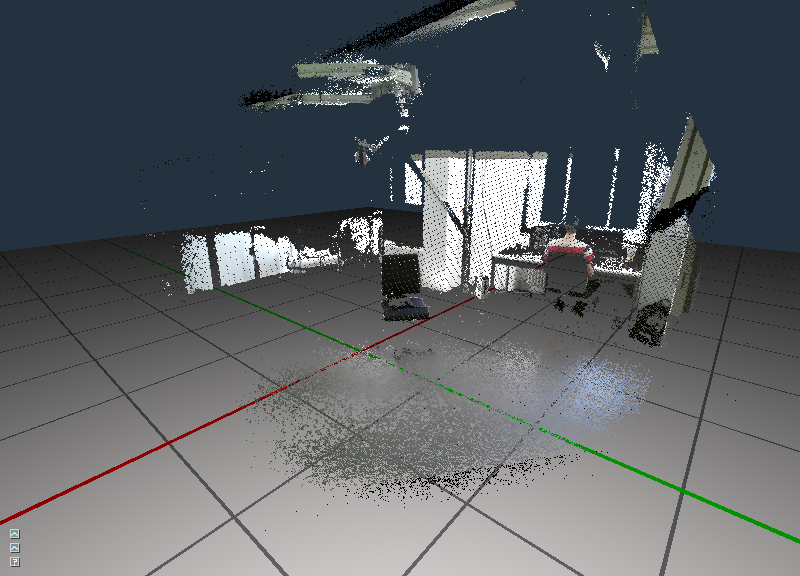
\includegraphics[width=0.7\paperwidth]{img/CloudPCViewer}};
	\end{tikzpicture}
	\end{center}
\end{frame}
\begin{frame}
    \frametitle{Problemstellung} 
    \begin{center}
	\begin{tikzpicture}
  		\node (img1) {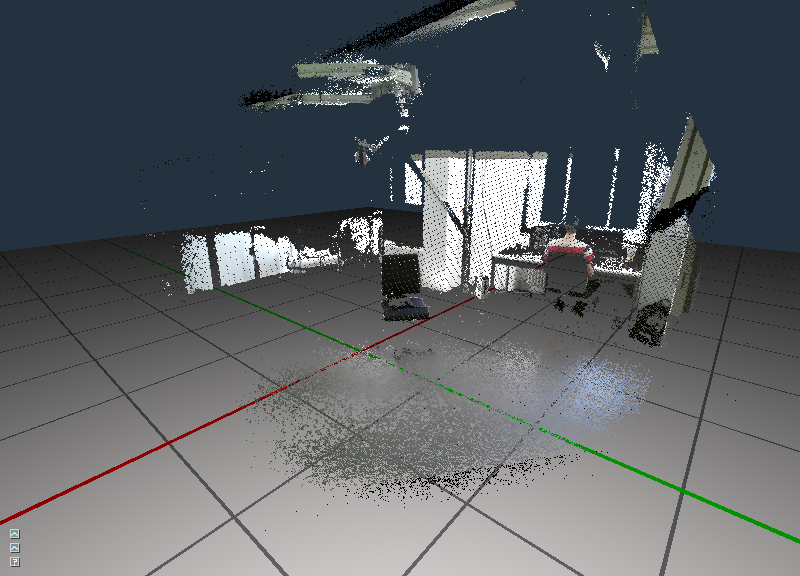
\includegraphics[width=0.7\paperwidth]{img/CloudPCViewer}};
  		\node (img2) at (img1.center) {
\includegraphics[width=0.3\paperwidth]{img/unreal-engine-4-logo}};
	\end{tikzpicture}
	\end{center}
\end{frame}

\begin{frame}
	\frametitle{Microsoft Kinect v2.0} 
	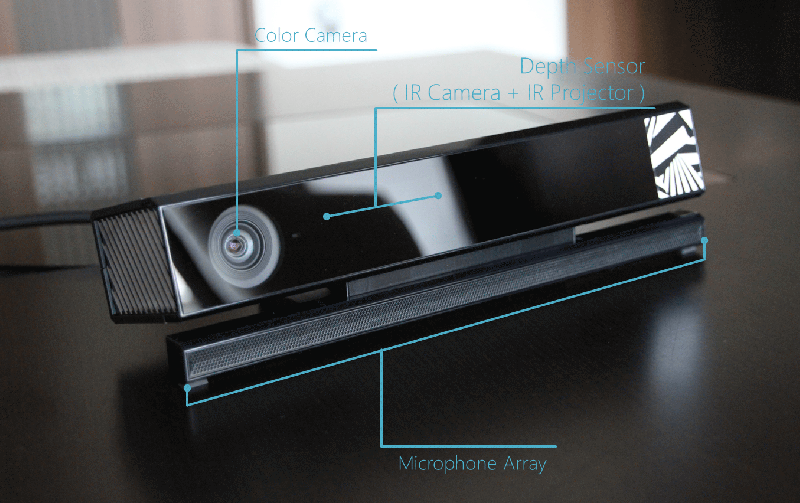
\includegraphics[width=0.7\paperwidth]{img/Kinectv2}
\end{frame}

\begin{frame}
	\frametitle{Kinect 4 Windows v2.0 Plugin} 
	\begin{itemize}
		\item Erlaubt es eine Kinect auszulesen und zu importieren
		\item Liest die Kinect über den Treiber aus $\Rightarrow$ Kinect RE und SDK erforderlich
		\item Importiert die Bilder als Texturen
		\item Achtung beim kompilieren
		\item \movie[externalviewer]{Video}{img/Kinect4Windows.WMV}
	\end{itemize}

\end{frame}

\begin{frame}
	\frametitle{PCViewer} 
	\begin{itemize}
		\item Client liest Kinect aus und versendet diese auf Anforderung an Server
		\item Server sammelt Daten ein
		\item Es gibt 4 Kinects in jeder Ecke des Holodecks ...
		\pause
		\item ... und auch für jede einen Rechner
		\item Der PCViewer kann bereits Point Clouds anzeigen
		\item \movie[externalviewer]{Video}{img/PCViewerVid.WMV}
		\pause
		\item Das 10.000 Cities Projekt benutzt ihn bereits
	\end{itemize}
\end{frame}

\begin{frame}
	\frametitle{Auslesen der Kinect Streams} 
	\begin{itemize}
		\item Verbindung zur Kinect prüfen
		\item Auslesefunktion des PCViewer aufrufen
		\item Unreal Engine arbeitet mit TArrays, PCViewer mit Puffern
		\item Z.B. Farben in drei uint8 Werten kodiert, Unreal möchte eine FColor
	\end{itemize}
	\begin{center}
		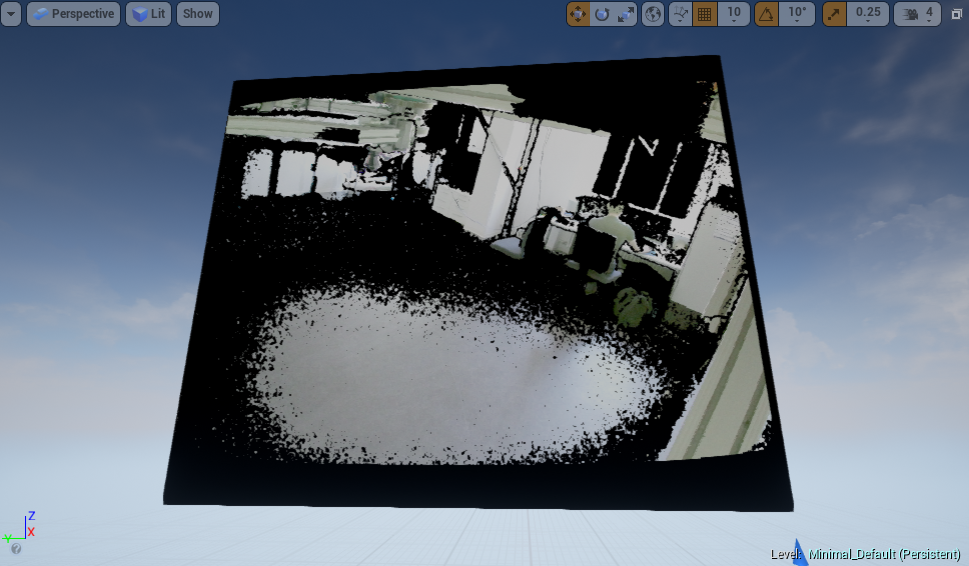
\includegraphics[height=0.4\paperheight]{img/2DColor}
		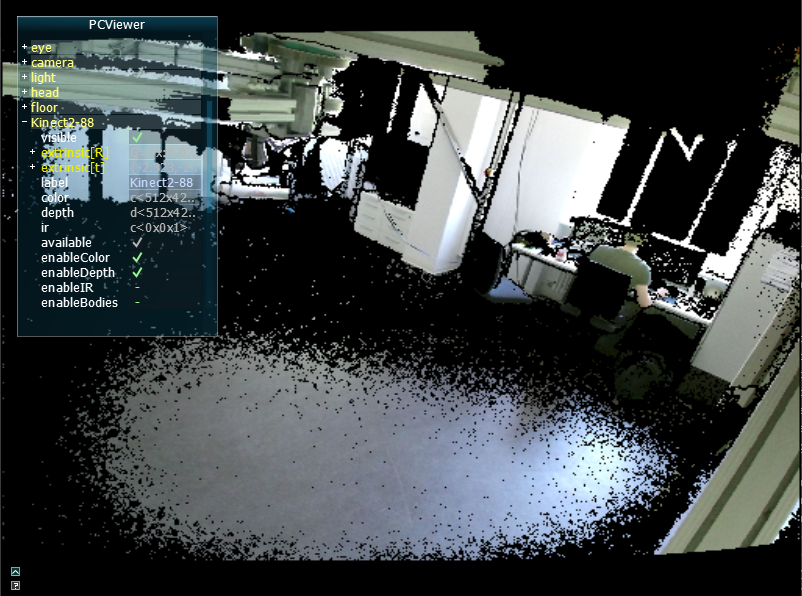
\includegraphics[height=0.4\paperheight]{img/2DColorPCViewer}
	\end{center}
\end{frame}

\begin{frame}
	\frametitle{Berechnen der 3D Position} 
Bildpunkt: $\begin{bmatrix}
u \\
v \\
\gamma
\end{bmatrix}
= \begin{bmatrix}
f_u & 0 & c_u  \\
0 & f_v & c_v  \\
0 & 0 & 1  
\end{bmatrix}
\times
\begin{bmatrix}
y_1 \\
y_2 \\
y_3
\end{bmatrix}$\\
\pause
3D (Ursprung): $\begin{bmatrix}
y'_1 \\
y'_2 \\
y'_3
\end{bmatrix}
= \begin{bmatrix}
f_u & 0 & c_u  \\
0 & f_v & c_v  \\
0 & 0 & 1  
\end{bmatrix}^{-1}
\times
\begin{bmatrix}
u \\
v \\
1
\end{bmatrix}
\times
\gamma
$
\end{frame}

\begin{frame}
	\frametitle{Berechnen der 3D Position} 
		Bildpunkt: 
		$\begin{bmatrix}
		u \\
		v \\
		\gamma
		\end{bmatrix}
		= 
		I
		\times
		\begin{bmatrix}
		y_1 \\
		y_2 \\
		y_3
		\end{bmatrix}$\\

		3D (Ursprung): 
		$\begin{bmatrix}
		y'_1 \\
		y'_2 \\
		y'_3
		\end{bmatrix}
		= 
		I^{-1}
		\times
		\begin{bmatrix}
		u \\
		v \\
		1
		\end{bmatrix}
		\times
		\gamma
		$ \\[1cm]
			
		3D Punkt:
		$\begin{bmatrix}
		y_1 \\
		y_2 \\
		y_3
		\end{bmatrix}
		= 
		E
		\times
		\begin{bmatrix}
		y'_1 \\
		y'_2 \\
		y'_3
		\end{bmatrix}$
\end{frame}

\begin{frame}
	\begin{center}
		\frametitle{Beispiel} 
		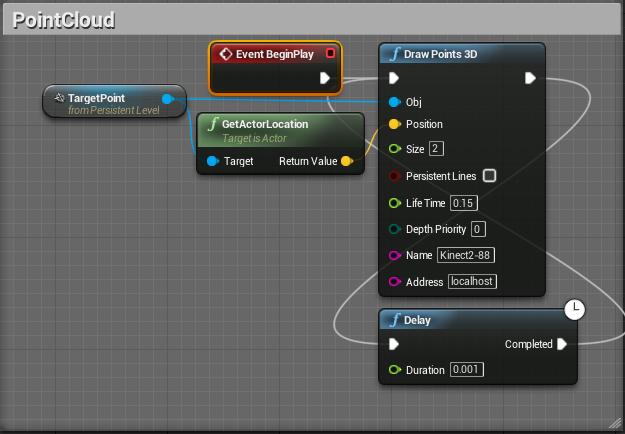
\includegraphics[width=0.8\paperwidth]{img/CloudBP}
	\end{center}

\end{frame}

\begin{frame}
	\frametitle{Ergebnis} 
	\begin{itemize}
		\item Nun an jede 3D Position einen farbigen Pixel zeichnen
		\item Dabei schwarze Pixel und Pixel ohne Tiefe auslassen
		\item \movie[externalviewer]{Video}{img/KinectCloudVid.WMV}
	\end{itemize}
	\begin{center}
		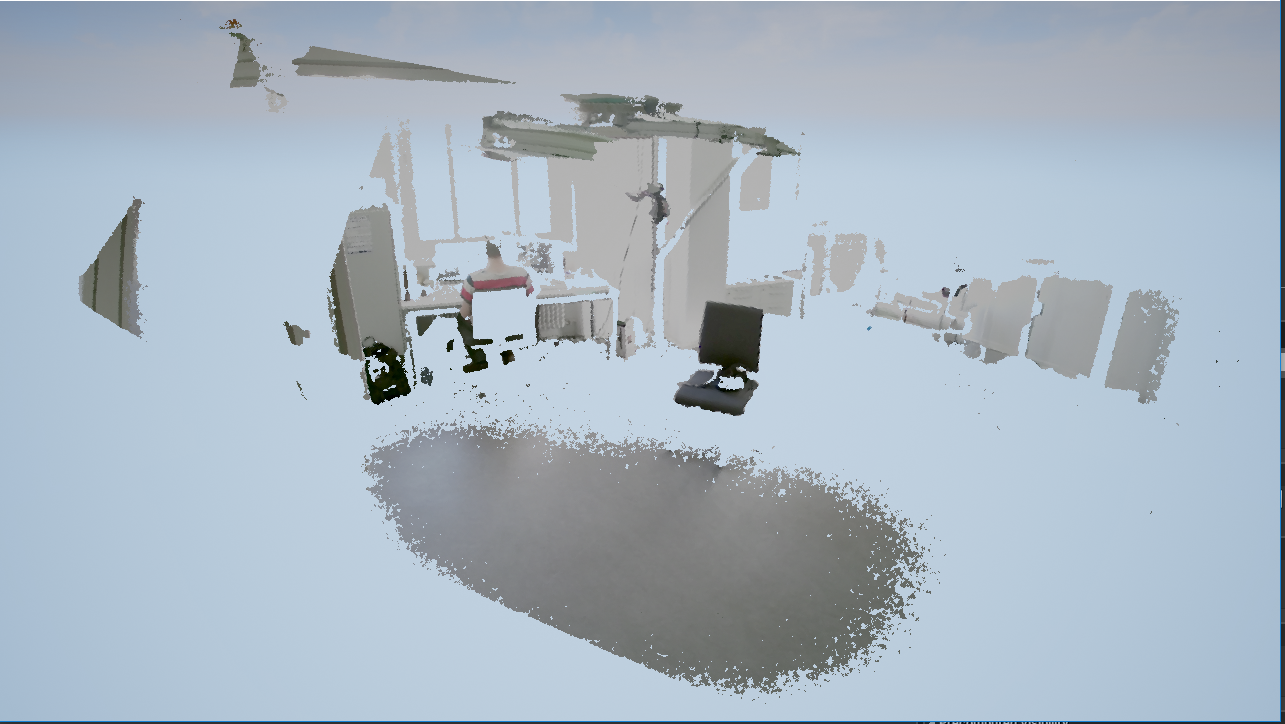
\includegraphics[height=0.37\paperheight]{img/Cloud}
		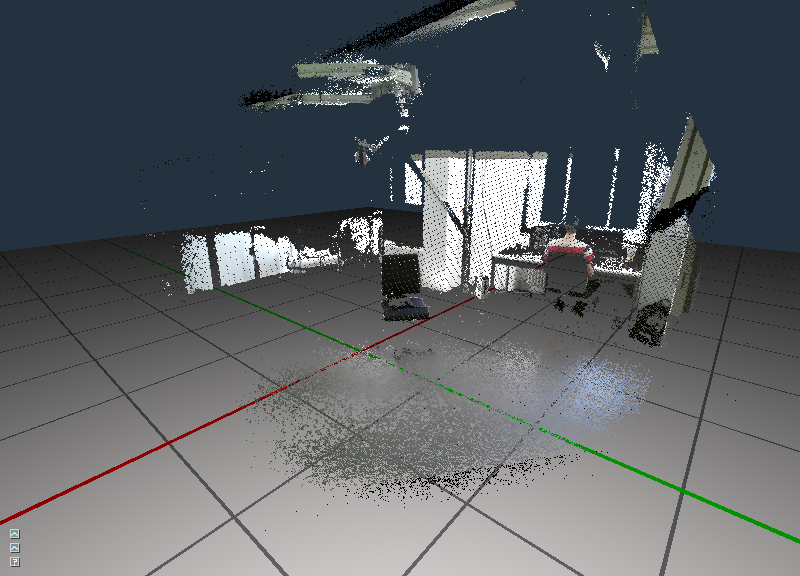
\includegraphics[height=0.37\paperheight]{img/CloudPCViewer}
	\end{center}
\end{frame}

\begin{frame}
	\frametitle{Implementierte Methoden und Fazit} 
	\begin{center}
		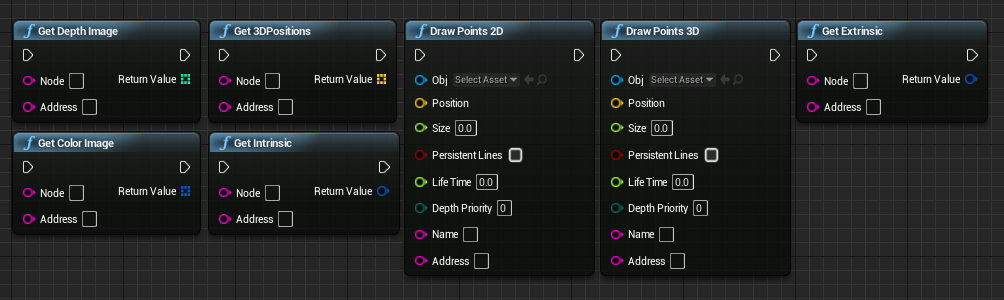
\includegraphics[height=0.37\paperheight]{img/AllFunctionsBP}
	\end{center}
	\begin{itemize}
		\item Erfolgreiche Übertragung!
		\item Funktionierender Prototyp
		\item Überraschend viele Umwandlungen notwendig
		\item Performancekritische Aufgabe $\Rightarrow$ Optimierungspotential
		\item Zeichnen sehr aufwändig $\Rightarrow$ verwenden von Particles
	\end{itemize}
\end{frame}


% Final page
\begin{frame}{~}
	\begin{center}
		\huge{Danke für Ihre Aufmerksamkeit}
	\end{center}
\end{frame}

\end{document}

